\chapter{Structure}
\label{chap:structure}
The flowchart presented in the introduction of this document 
represents the macro objects of the library and reflects 
closely the capabilities of \Atlas. We subdivide this 
chapter in various sections, each of them representing one 
of the objects in \fig{fig:intro-schematics}. The order in 
which these objects will be presented starts from the grid 
and closes with the numerics. Note that some simple examples 
are provided as part of this user-guide in \parte{p:core-functionalities}.



\section{Grid}
The Grid object relies on a hierarchical inheritance tree 
as shown in \fig{fig:grids}. It is responsible for generating 
a list of coordinates representing the points of a given grid. 
The grids that \Atlas constructs can be \textit{Global} or 
\textit{Local}. The first typology of grid represents a complete 
spherical grid, while the second typology represents a limited 
area of the sphere. Both Global and Local grids can be either 
structured or unstructured. In \fig{fig:grids} we show the 
various derived classes of the Grid object and its current 
capabilities.
%
\begin{figure}[htb]
\centering
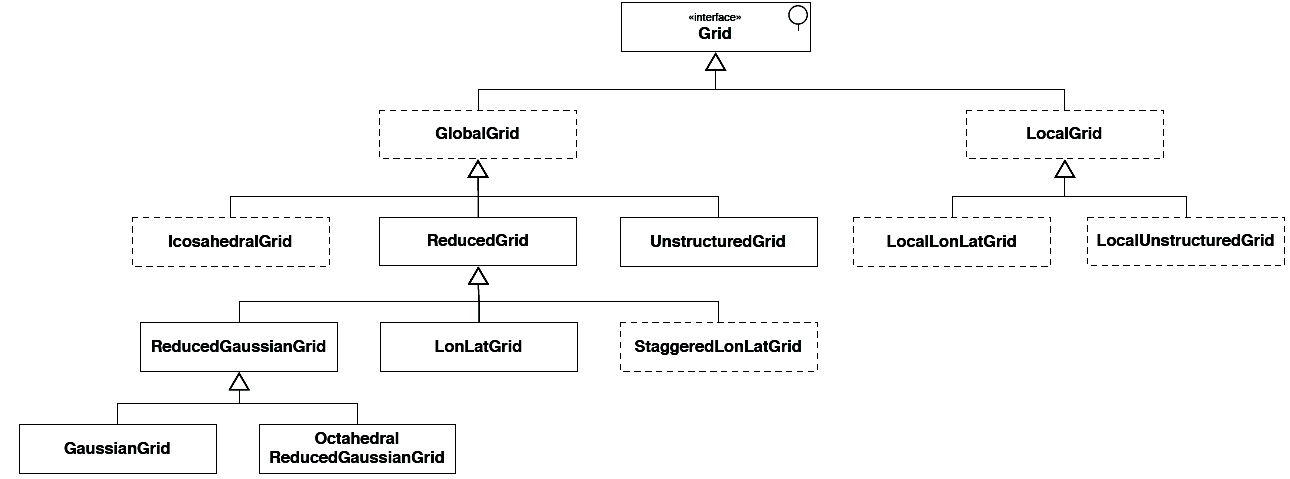
\includegraphics[scale=0.3]{imgs/grids.png}
\label{fig:grids}
\caption{Grid object derived classes and capabilities}
\end{figure}
%
In particular, a Global grid has several possible implementations, 
such as the following derived types: IcosahedralGrid, ReducedGrid 
and UnstructuredGrid. The ReducedGrid has three additional derived 
types: ReducedGaussianGrid, LonLatGrid and StaggeredLonLatGrid.
The ReducedGaussianGrid, in turn, can be either a GaussianGrid 
or an OctahedralReducedGaussianGrid.

We note that the object-oriented construction of the Grid 
object allows one to add any other grid that might be of 
interest without disrupting the existing grid workflow.



\section{Mesh}
The Mesh object is responsible for generating a distributed 
mesh starting from a given grid. The associated workflow is 
depicted in \fig{fig:mesh1}.

The mesh is constructed using the class MeshGenerator that 
takes as an input the grid (optionally a grid distribution 
that is defined as ...).
The MeshGenerator object is, in turn, composed by a ReducedGridMeshGenerator 
and a Delaunay object. The first ..., while the second ...
%
\begin{figure}
\centering
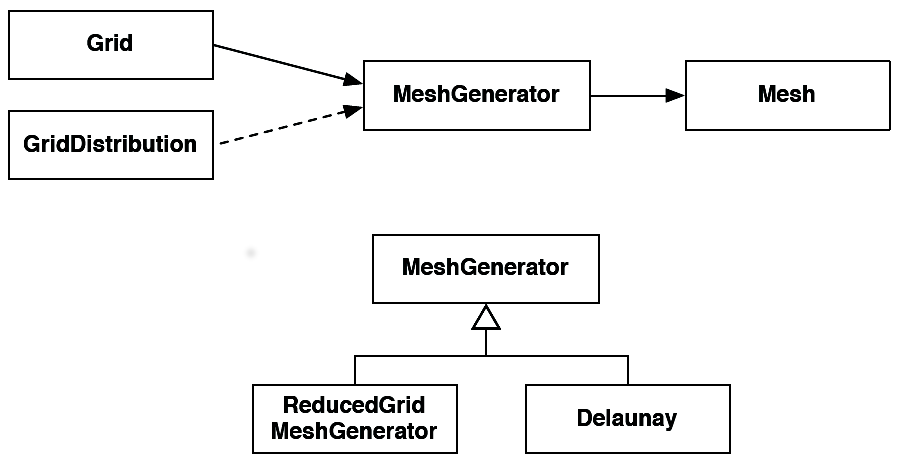
\includegraphics[scale=0.25]{imgs/mesh1.png}
\label{fig:mesh1}
\caption{Mesh workflow}
\end{figure}
% 
In \fig{fig:mesh2} we show the composition of the mesh object.
%
\begin{figure}
\centering
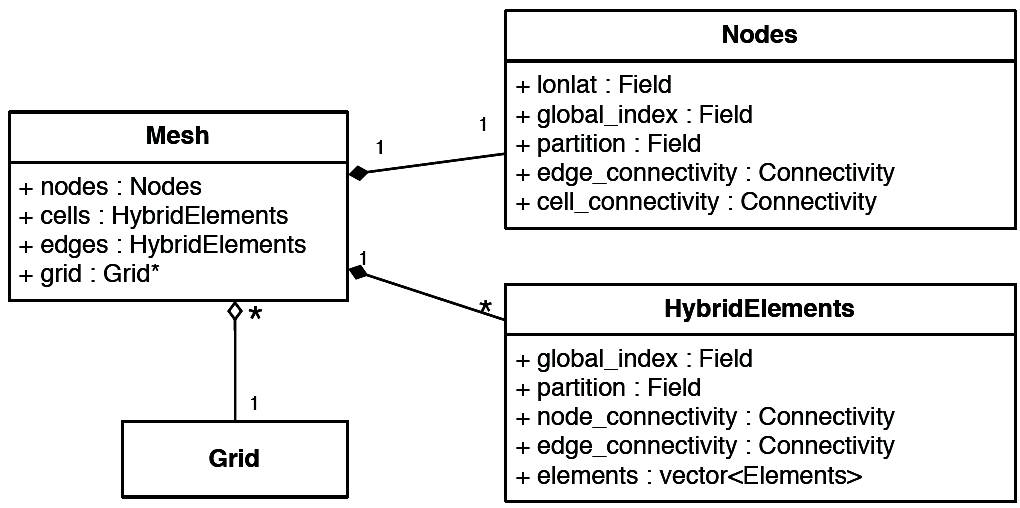
\includegraphics[scale=0.25]{imgs/mesh2.png}
\label{fig:mesh2}
\caption{Mesh object composition}
\end{figure}
%
In particular, the nodes and elements define node connectivities 
and the mesh is constructed to be generically unstructured - i.e. 
there are no specific requirements for the mesh to be structured.
%
\begin{warningbox}
Note that a mesh is not equal to a grid. The grid is a list of points 
without connectivity, while a mesh is a list of nodes with specific 
connectivity rules. Note also that, in \Atlas, the number of points 
of a grid is generally different from the number of nodes of a mesh.
\end{warningbox}
%

\section{Field and FieldSet}
Field objects encapsulate given fields, such as the wind speed 
or the pressure, and they can be grouped into FieldSets. 
The structure of the field object is depicted in \fig{fig:field}.
%
\begin{figure}
\centering
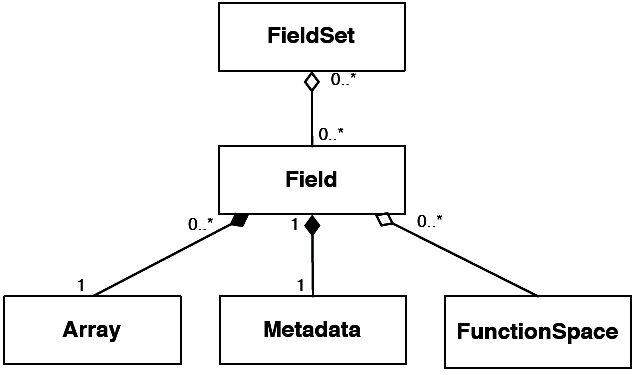
\includegraphics[scale=0.25]{imgs/field.png}
\label{fig:field}
\caption{Field and FieldSet object composition}
\end{figure}
%
In particular the Field object is composed of three elements:
the Array object, the Metadata object and the FunctionSpace 
object. The Array object contains the actual memory where the 
data is stored, while the Metadata object is instead responsible 
for the description of a given field. Finally the FunctionSpace
object allows one to define a field on a particular function 
space (such as a spectral space, grid point space, or a spectral 
element space).


 
\section{FunctionSpace}
The FunctionSpace object allows a concrete representation 
of the fields defined through the object Field. In 
\fig{fig:functionspace} we show the diagram of the 
FunctionSpace object.
%
\begin{figure}
\centering
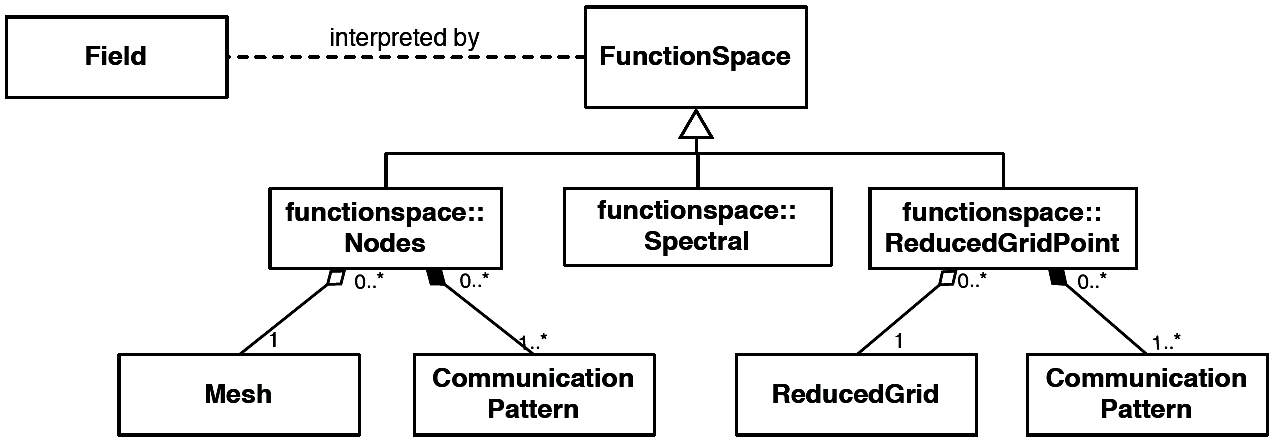
\includegraphics[scale=0.25]{imgs/functionspace.png}
\label{fig:functionspace}
\caption{FunctionSpace object diagram}
\end{figure}
%
There exist a variety of possible function spaces. Functionspaces 
have knowledge of how a field is discretised in the domain and 
can be used to interpret related fields. Examples include the 
spectral function space, where a spectral representation of a 
field is employed, the spectral element space, where elemental 
spectral functions are used to describe a field, etc.



\section{Numerics}
The numerics in Atlas is strictly related to the FunctionSpace 
object. In particular, the FunctionSpace object dictates the 
construction of the numerical operators.
A concrete implementation of a numerical operator is the Nabla 
implementation for edge-based finite volume methods. This operator 
uses the functionspace edge-based finite volume to define the 
the implementation of operators for the gradient, curl, divergence
and Laplacian. This structure is depicted in \fig{fig:numerics}.
%
\begin{figure}
\centering
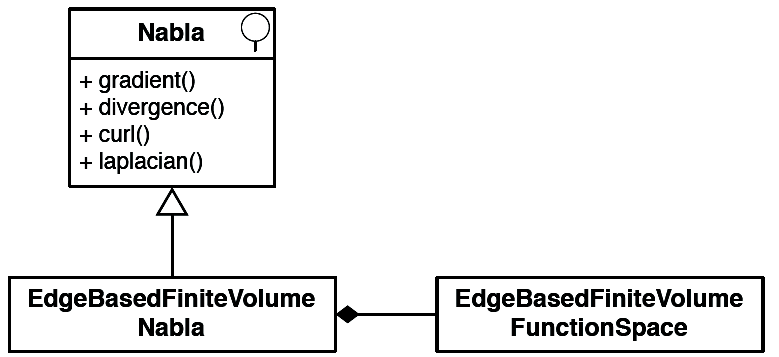
\includegraphics[scale=0.25]{imgs/numerics.png}
\label{fig:numerics}
\caption{Numerics object composition}
\end{figure}
%


\section{Utilities}
A number of utilities is also available with the library. These include 
pre- and post-processing tools, mpi communication, error and exception 
handling, runtime behaviour, etc.

